\imprimircapa	% Capa
\imprimirfolhaderosto*	% Folha de rosto. * indica que haverá a ficha bibliográfica

\begin{fichacatalografica}
	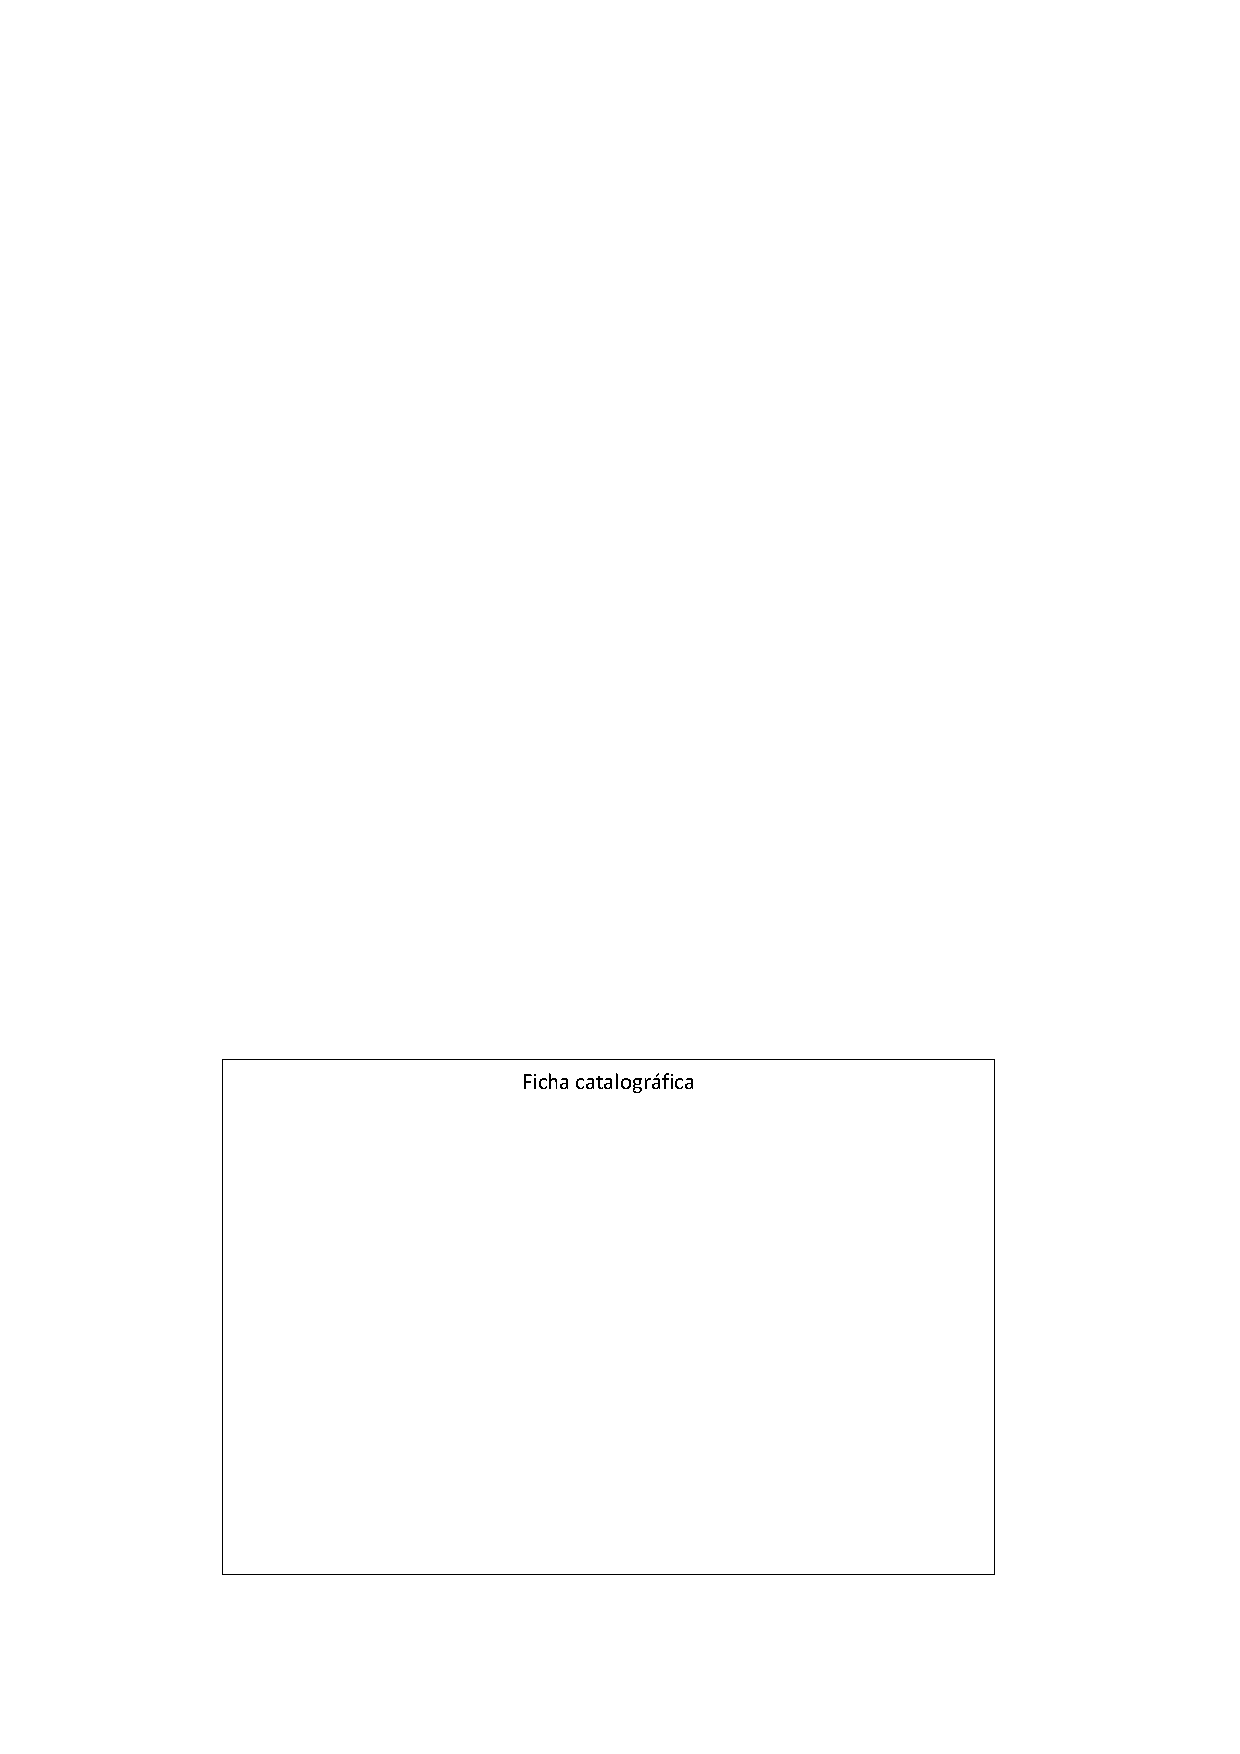
\includepdf{ficha_catalografica.pdf}
\end{fichacatalografica}

\begin{folhadeaprovacao}
	
	\begin{center}
		{\ABNTEXchapterfont\large\imprimirautor}
		
		\vspace*{\fill}\vspace*{\fill}
		\begin{center}
			\ABNTEXchapterfont\bfseries\Large\imprimirtitulo
		\end{center}
		\vspace*{\fill}
		
		\hspace{.45\textwidth}
		\begin{minipage}{.5\textwidth}
			\imprimirpreambulo
		\end{minipage}%
		\vspace*{\fill}
	\end{center}
	
	Trabalho aprovado. \imprimirlocal, 31 de dezembro de 2020:
	
	\assinatura{\textbf{\imprimirorientador} \\ Orientador} 
	\assinatura{\textbf{\imprimircoorientador} \\ Coorientador} 
	\assinatura{\textbf{Professor} \\ Convidado 1}
	\assinatura{\textbf{Professor} \\ Convidado 2}
	
	\begin{center}
		\vspace*{0.5cm}
		{\large\imprimirlocal}
		\par
		{\large\imprimirdata}
		\vspace*{1cm}
	\end{center}
	
\end{folhadeaprovacao}

% Resumo em português
\setlength{\absparsep}{18pt} % Ajusta o espaçamento dos parágrafos do resumo
\begin{resumo}
	A mudança de paradigma na indústria referente às recentes modificações em relação às tecnologias de manufatura é chamada de Indústria 4.0 (I4.0). Nesse novo conceito, redes inteligentes de máquinas e processos para indústria com o respaldo de Tecnologias da Informação e Comunicação (TIC) passam a proporcionar um alto nível de automação e intercâmbio de informações entre equipamentos, produtos e demais atores em um ambiente de manufatura.
	Este trabalho aborda uma proposta de desenvolvimento dos detalhes do Modelo de Arquitetura de Referência para a Indústria 4.0 (RAMI4.0), especificamente por meio da introdução do conceito de Memória Digital do Produto (MDP) ao eixo horizontal ``Ciclo de Vida e Cadeia de Valor'', de forma a se aperfeiçoar a elaboração dessa arquitetura, proporcionando mais robustez ao modelo para uma futura adoção generalizada por parte de empresas por todo o mundo.
	O estudo aborda uma nova estrutura de compartilhamento da MDP do ativo por meio de \textit{Web Services} composta por quatro elos: O Componente I4.0, o Repositório, a MDP e o Cliente. A proposta de estrutura é tratada com base no RAMI4.0 e visa propiciar o surgimento de novos cenários de criação de valor no contexto da I4.0 e incentivar a geração de novos modelos de negócio baseado em dados.
	
	\textbf{Palavras-chave}: Indústria 4.0. RAMI4.0. Memória digital do produto. Arquitetura Orientada a Serviços (SOA). Cadeia de Suprimentos.
\end{resumo}

% Resumo em inglês
\begin{resumo}[Abstract]
	\begin{otherlanguage*}{english}
		This is the english abstract.
		
		\vspace{\onelineskip}
		
		\noindent 
		\textbf{Keywords}: Industry 4.0. RAMI4.0. Digital product memory. Value Chain. Product life cycle. 
	\end{otherlanguage*}
\end{resumo}

% Lista de ilustrações
\pdfbookmark[0]{\listfigurename}{lof}
\listoffigures*
\cleardoublepage

% Lista de tabelas
% ---
\pdfbookmark[0]{\listtablename}{lot}
\listoftables*
\cleardoublepage

% Lista de abreviaturas e siglas
\begin{siglas}
	\item[AAS] \textit{Asset Administration Shell} (Camada Administrativa do Ativo)
	\item[API] \textit{Application Programming Interface} (Interface de Programação de Aplicação)
	\item[BD] Banco de Dados
	\item[BI] \textit{Business Intelligence} (Inteligência Empresarial)
	\item[CS] Cadeia de Suprimentos
	\item[CV] Cadeia de Valor
	\item[CVP] Ciclo de Vida do Produto
	\item[GCVP] Gestão do Ciclo de Vida do Produto
	\item[GI] Gestão da Informação
	\item[I4.0] Indústria 4.0
	\item[IIoT] \textit{Industrial Internet of Things} (Internet das Coisas Industrial)
	\item[IoT] \textit{Internet of Things} (Internet das Coisas)
	\item[MDP] Memória Digital do Produto
	\item[OSI] \textit{Open System Interconnection} (Interconexão aberta de sistemas)
	\item[RAMI4.0] \textit{Reference Architectural Model Industrie 4.0} (Modelo de Arquitetura de Referência para a Indústria 4.0)
	\item[REST] \textit{Representational State Transfer} (Transferência Representacional de Estado)
	\item[RFID] (\textit{Radio-Frequency IDentification}) (Identificação por Radiofrequência)
	\item[SOA] \textit{Service Oriented Architecture} (Arquitetura Orientada a Serviços)
  	\item[TIC] Tecnologia da Informação e Comunicação
  	\item[UUID] \textit{Universal Unique IDentifier} (Identificador Único Universal)
  	\item[WS] \textit{Web Service} (Serviço Web)
  	\item[WSD] \textit{Web Services Description} (Descrição do Serviço Web)
  	\item[WSDL] \textit{Web Services Description Language} (Linguagem de Descrição de Serviços Web)
\end{siglas}

% Sumário
\pdfbookmark[0]{\contentsname}{toc}
\tableofcontents*
\cleardoublepage
